\documentclass[11pt,a4paper,oneside]{report}

% MARK - Packages
\usepackage{amsmath}
\usepackage{siunitx}
\usepackage[x11names,table,xcdraw]{xcolor}
\usepackage{natbib}
\usepackage{mathrsfs}
\usepackage{color} %red, green, blue, yellow, cyan, magenta, black, white
\usepackage[scr]{rsfso}
\usepackage{graphicx}
\usepackage{listings}
\usepackage{bigfoot}
\usepackage[numbered,framed]{matlab-prettifier}
\usepackage{titletoc,tocloft}
\usepackage{setspace}
\usepackage{natbib}
\usepackage[a4paper,left=2cm,right=2cm,top=2.5cm,bottom=2.5cm]{geometry}
\usepackage[siunitx]{circuitikz}
\usepackage{framed}
\usepackage{quoting}
\usepackage{xlop}
\usepackage{float}
\usepackage{titlesec}
\usepackage{csvsimple}
\usepackage{tikz}
\usepackage{caption}
\usepackage{subcaption}
\usepackage[numbered,framed]{matlab-prettifier}
\usepackage{physics} % for 'pdv' macro
\usepackage{multicol}
\usepackage{courier}
\usepackage{sourcecodepro}
\usepackage[normalem]{ulem}
\usepackage{pgfplots}
\usepackage[bookmarks]{hyperref}
\pgfplotsset{width=10cm,compat=1.9}
\usepackage{url}
\usepackage{import}
\useunder{\uline}{\ul}{}

% MARK - Metadata
\author{
  Jesse Onolememen\\
  20344056
  \and
  Omar Issa\\
  19204747
  \and
  David Jones\\
  20329631
}
\title{
  \textbf{EEEN30150 Modelling \& Simulation} \\
  \large Minor Project 2 (MP2): Dynamic Equations \\
  \textit{Team 42}
  }
\date{\today}
\onehalfspacing
\setcounter{secnumdepth}{4}
\setcounter{tocdepth}{3}
\graphicspath{../exports}
\bibliographystyle{agsm}
\numberwithin{equation}{section}
\setlength{\parindent}{0pt}

% MARK - Quotations
\colorlet{shadecolor}{LavenderBlush2}
\colorlet{framecolor}{lightgray}
\renewenvironment{shaded*}{%
  \def\FrameCommand{\setlength{\FrameRule}{2pt}\fboxsep=\FrameSep \fcolorbox{framecolor}{shadecolor}}%
  \MakeFramed {\advance\hsize-\width \FrameRestore}}%
 {\endMakeFramed}


\newenvironment{shquote}
 {\begin{shaded*}
  \quoting[leftmargin=0pt, vskip=0pt]
 }
 {\endquoting
 \end{shaded*}
}

% Title format
\titleformat{\chapter}[display]
  {\normalfont\bfseries}{}{0pt}{\Huge}
\titlespacing*{\chapter}{0pt}{0pt}{12pt}

% MARK - Custom Commands
\setcounter{section}{0}
\renewcommand{\thesection}{\arabic{section}}
\newcommand{\lpt}[1]{\mathcal{L}\{#1\}}
\newcommand{\sbracket}[1]{\left[#1 \right]}
\newcommand{\bracket}[1]{\left(#1 \right)}

\def\therefore{\boldsymbol{\text{ }
\leavevmode
\lower0.4ex\hbox{$\cdot$}
\kern-.5em\raise0.7ex\hbox{$\cdot$}
\kern-0.55em\lower0.4ex\hbox{$\cdot$}
\thinspace\text{ }}}

% Listings
\lstset{style=Matlab-editor}
%\setmonofont{Lucida Console}[Scale=MatchLowercase] % select a suitable monospaced font
\lstset{basicstyle=\fontsize{9}{9}\ttfamily,breaklines=true}
\lstset{framextopmargin=50pt,frame=bottomline}

\usepackage{xcolor}
\definecolor{maroon}{cmyk}{0, 0.87, 0.68, 0.32}
\definecolor{halfgray}{gray}{0.55}
\definecolor{ipython_frame}{RGB}{207, 207, 207}
\definecolor{ipython_bg}{RGB}{247, 247, 247}
\definecolor{ipython_red}{RGB}{186, 33, 33}
\definecolor{ipython_green}{RGB}{0, 128, 0}
\definecolor{ipython_cyan}{RGB}{64, 128, 128}
\definecolor{ipython_purple}{RGB}{170, 34, 255}


%%
%% Python definition (c) 1998 Michael Weber
%% Additional definitions (2013) Alexis Dimitriadis
%% modified by me (should not have empty lines)
%%
\lstdefinelanguage{MatLab}{
    basicstyle=\footnotesize,
    keywordstyle=\color{ipython_green}\ttfamily,
}

% Matrix columns
\setcounter{MaxMatrixCols}{15}
\newcommand{\nodecirc}[1]{\textcircled{#1} \hspace{0.15cm} \triangleright \hspace{0.25cm}}

% MARK - Begin Document

\begin{document}

% S; Front Page
\maketitle

% S; Plagarism Declaration
\leavevmode%
\vfill\noindent
\begin{center}
  \textbf{Declaration of Authorship}
\end{center}
I declare that all material in this assessment is my our work except where there is clear acknowledgement and appropriate reference to the work of others.

\vspace*{4em}\noindent
\hfill%
\begin{tabular}[t]{c}
  \rule{10em}{0.4pt} \rule{10em}{0.4pt} \rule{10em}{0.4pt}\\ Signed
\end{tabular}%
\hfill%
\begin{tabular}[t]{c}
\rule{10em}{0.4pt}\\ Date
\end{tabular}%
\hfill
\strut
\vspace{4em}


% S; Table of Contents
\newpage
\setlength{\cftsubsecindent}{1.5cm}
\setlength{\cftsubsubsecindent}{1.5cm}
\doublespacing
\tableofcontents
\onehalfspacing

% S; Sections
\section*{Problem 2.1: A Simple Power Supply}
A simple power supply is presented for analysis. 
\begin{figure}[H]
    \centering
    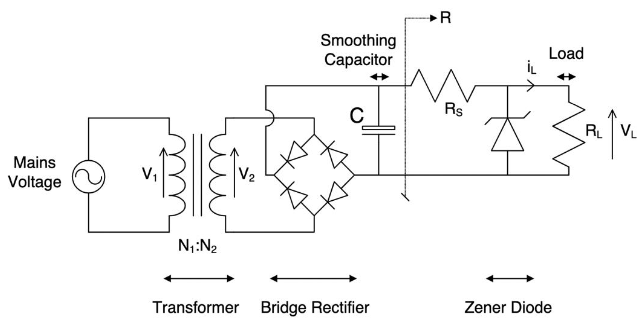
\includegraphics[width=\textwidth]{graphics/powersupply.png}
    \caption{Simple power supply}
    \label{fig:powersupply}
\end{figure}
The power supply is terminated by a multi-mode load resistor modelled by its Thevenin equivalent circuit. The circuit has multiple modes of operation depending on the switching of its devices. The circuit is presented below.
\begin{figure}[H]
    \centering
    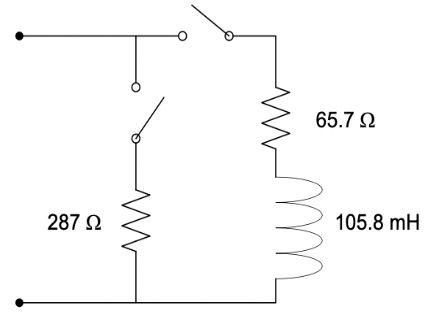
\includegraphics[width=8cm]{graphics/multimode_load.png}
    \caption{Multi-mode load}
    \label{fig:multimode_load}
\end{figure}
The performance of the circuit is to be determined for all modes of operation. A mathematical model of the circuit is derived for use in numerical analysis and simulation. A visualisation is presented at the end with the results.
\section{Modelling}
A model of each individual circuit component is fabricated. This is used to provide a model of the circuit as a whole, using nodal analysis methods .i.e. Krichoff's Laws

\subsection{Component Values}
The values of the circuit components are presented in the table below. Where there is an applicable tolerance level, the maximum and minimum values are shown. 
\begin{table}[H]
    \centering
    \begin{tabular}{|c|c|c||c|c|}\hline
        & Value & \% Tolerance & \textbf{Maximum} & \textbf{Minimum} \\\hline
       $C$ & $0.0022 F$ & $20\%$ & $0.00264F$ & $0.00176F$ \\
       $R_s$ & $300\Omega$ & $10\%$ & $330\Omega$ & $270\Omega$ \\
       $R_{L_1}$ & $65.7\Omega$ & $0\%$ & $65.7\Omega$  & $65.7\Omega$ \\
       $R_{L_2}$ & $287\Omega$ & $0\%$ & $287\Omega$ & $287\Omega$ \\
       $L_L$ & $0.01058 H$ & $0\%$ & $0.01058 H$ & $0.01058 H$ \\\hline
    \end{tabular}
    \caption{Circuit component values and their variances}
    \label{tab:component_values}
\end{table}

\subsection{Component Modelling}
Each individual component in the circuit must be represented analytically. Circuit components are assumed to be ideal, .i.e. there is an absence of source resistance and or impedance. The model does not account for inexactitudes in component values that may be realised in a practical implementation. 

\subsubsection{Voltage Source} The voltage source is modelled as an ideal AC voltage source. There is no source impedance, thus, we assume that the source generates the exact amount of voltage across its terminals. 
\begin{equation}
    \begin{split}
        V_{\text{in}} &= V_{\text{rms}}\sqrt{2}\text{sin}(\omega t + \phi)
            \\ &= 230\sqrt{2}\text{sin}(100\pi t)V
    \end{split}
\end{equation}
where $V_{\text{rms}}$ is the rms voltage, $\omega = 2\pi f$ is the angular frequency

\subsubsection{Capacitor} The capacitor is modelled as an ideal capacitor that does not dissipate energy. The current across the capacitor is given by:
\begin{equation}
    i = C \frac{dV}{dt}
\end{equation}
where $C$ is the capacitance in Farads (F), $\frac{dV}{dt}$ is the rate of change of voltage $\left(\frac{V}{s}\right)$

\subsubsection{Inductor} The inductor is modelled as an ideal inductor whose voltage is given by:
\begin{equation}
    V = L\frac{di}{dt}
\end{equation}
where $L$ is the inductance in Henry's, $\frac{di}{dt}$ is the rate of current change
\subsubsection{Resistor} The resistor is modelled as an ideal resistor whose voltage is given by Ohm's law
\begin{equation}
    V=IR
\end{equation}
where $V$ is the voltage (V), $I$ is the current (A) and $R$ is the resistance ($\Omega$)

\subsubsection{Switch} The switch is modelled as an ideal switch without any source resistance. The switch can be represented using a binary state .i.e. on or off. It is assumed that there is no propagation delay in the change of state and the effects are immediate. 

\subsubsection{Transformer} The transformer is assumed to be ideal with a turns ratio of $20:1$. The voltage at either side of the transformer can be determined from its common ideal representation
\begin{equation}
    \frac{V_1}{V_2} = \frac{N_1}{N_2}
\end{equation}
where $N_1=20$ is the number primary turns, $N_2=1$ is the number of secondary turns, $V_1$ is the primary voltage, $V_2$ is the secondary voltage.\\

The voltage at LV-side of the transformer is fed into the full-bridge rectifier. The secondary voltage $V_2$ is given by:
\begin{equation}
    V_2 = \frac{V_1N_2}{N_1}
\end{equation}

\subsubsection{Diode}
The four diodes in the circuit are configured to form a full bridge rectifier. It is assumed all four diodes are identical.

\paragraph{Shockley Ideal Diode}
The diodes can be modelled as a Shockley diode in series with bulk resistance. The Shockley diode model is a simplified model to describe the behaviour of a diode:

\begin{equation}
	I_D = I_s\left( e^{\frac{V_D}{\eta V_T}} - 1 \right) + \frac{V_d}{R_b}	\label{shockeyDiodeWithBulkResistance}
\end{equation}
where,
\begin{itemize}
	\item $I_D$ is the diode current
	\item $I_s$ is the saturation current
	\item $V_D$ is the voltage across the diode
	\item $\eta$ is the ideality factor
	\item $V_T$ is the thermal voltage (determined by $V_T = \frac{KT}{q}$)
	\item $R_b$ is the bulk resistance
\end{itemize}	

The Shockley diode presents a non-linear model of the diode's behaviour which complicates circuit analysis. A piece-wise linear approximation to the DC characteristic of the diode is used for simplicity.

\paragraph{Piece-wise Linear Approximation}
An ideal diode behaves as a switch–conducting current without any losses under forward bias, and completely blocking current under reverse bias. The biasing of a diode is determined by assessing whether the voltage drop across the diode is greater than its threshold voltage ($V_D \geq V_{th}$)

\subparagraph{Ideal Diode}
Assume that the diode is a silicon diode with a threshold voltage of $V_{th} = 0.7 V$.  The current across diode can be represented analytically as:
\begin{equation}
    i_d = \begin{cases}
        \infty \hspace{1cm} &V_d \geq 0.7V \\
        0 \hspace{1cm}   &V_d < 0.7V
    \end{cases}
    \label{eq:ideal_diode}
\end{equation}
\begin{figure}[H]
    \centering
    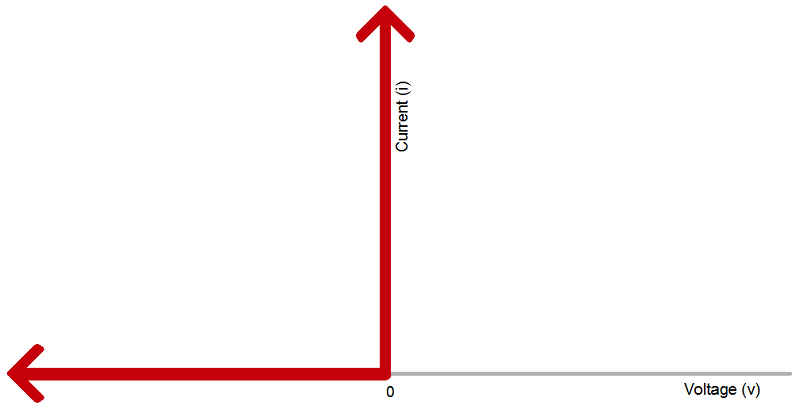
\includegraphics[width=10cm]{graphics/diode_iv.png}
    \caption{The ideal diode i-v characteristic. This graph assumes $V_{th}=0$}
    \label{fig:diode_iv_characterstic}
\end{figure}
Consider the behaviour of the diode inside the bridge rectifier. The diode is represented as a cell ($V_{th}$) in series with a resistor ($R_b$) and an ideal switch. The current flowing into the switch is represented by $i_d$. This is the piece-wise linear approximation of the diode.
\begin{figure}[H]
    \centering
    \begin{circuitikz} \draw
 	(0,7) to[diode,l=$V_d$,i=$i_d$] (0,0)
	(3,7) to[battery1, l=$V_{th}$] (3,6) 
	(3,6) to[R, l=$R_b$, i_=$i_d$] (3,2)
	(3,2) to[nos,o-o] (3,0);
\end{circuitikz}
    \caption{Piece-wise linear diode approximation of the ideal diode}
    \label{fig:piecewise_diode}
\end{figure}

Analytically $i_d$ can be described using Ohm's law and considering the voltage drop across $R_b$ 
\begin{equation}
    i_d = \begin{cases}
        \bracket{\frac{V_d - V_{th}}{R_b}} \hspace{1cm} &V_d \geq 0.7V \\
        0 \hspace{1cm}   &V_d < 0.7V
    \end{cases}
\end{equation}
This expression matches the expression for the ideal diode presented in Equation \ref{eq:ideal_diode}. 

\subsubsection{Determination of Maximum Current}
\subsubsection{Comparison to Shockley Diode}

\subsubsection{Zener Diode}

\subsection{Circuit Modelling}

\section{Numerical Analysis}
\subsection{Classic Runge-Kutta Method}

Belonging to a family of iterative methodologies, Runge-Kutta methods, particularly the fourth-order variant (RK4), serve as prominent tools for numerically addressing differential equations. RK4 finds widespread use due to its efficacy in generating solutions to ordinary differential equations (ODEs) that may otherwise be challenging or impractical to solve analytically.

The crux of the Runge-Kutta method lies in using derivative evaluations at several junctures within a designated time step to project an estimate for the function's value at the succeeding step. This is achieved by approximating the Taylor series up to the order of the step size, which is conventionally represented by 'h'.

To illustrate, for a first-order ODE defined as $y' = f(t, y)$, the application of RK4 to progress from time $t$ to $t + h$ would involve the following steps:

\begin{equation}
\begin{aligned}
k_1 &= h \cdot f(t, y), \\
k_2 &= h \cdot f(t + \frac{h}{2}, y + \frac{k_1}{2}), \\
k_3 &= h \cdot f(t + \frac{h}{2}, y + \frac{k_2}{2}), \\
k_4 &= h \cdot f(t + h, y + k_3), \\
y(t + h) &= y(t) + \frac{1}{6} \cdot (k_1 + 2k_2 + 2k_3 + k_4).
\end{aligned}
\end{equation}

In this instance, the calculated 'k' values represent estimations of the function's slope at diverse points within the time step. The method essentially involves crafting a weighted mean of these slopes to derive the next value.\\

Let us define the next step in the solution, $y_{n+1}$, by the equation
\begin{equation}
y_{n+1} = y_n + \frac{h}{6} (k_1 + 2k_2 + 2k_3 + k_4) \quad (3.1)
\end{equation}
Here, $h$ represents the increment in the value of $t$ at each step.

The coefficients $k_i$ denote the slopes at different points in the time step and are defined as follows:
\begin{equation}
f(t, y) = \frac{dy}{dt}\bigg|_{(t, y)} = y'(t, y) \quad (3.2)
\end{equation}
\begin{align*}
k_1 &= f(t_n, y_n), &\text{initial slope using Euler's method},\\
k_2 &= f \left(t_n + \frac{h}{2}, y_n + \frac{k_1}{2}\right), &\text{slope at the midpoint using $y$ and $k_1$},\\
k_3 &= f \left(t_n + \frac{h}{2}, y_n + \frac{k_2}{2}\right), &\text{slope at the midpoint using $y$ and $k_2$},\\
k_4 &= f(t_n + h, y_n + k_3), &\text{slope at the end of the interval using $y$ and $k_3$}.
\end{align*}

These coefficients are defined for $n = 0, 1, 2, 3, \ldots$ . It can be clearly observed that this method bestows higher weights to the midpoint slopes during the computation of their weighted average.

RK4 can be conveniently extended to cater to systems of ordinary differential equations by replacing $y_n$ with the corresponding vector of unknowns.

Four distinctive scenarios are to be considered, each featuring diverse loads connected to the DC rectifier. These will be thoroughly analyzed individually. In the derivation of the equations, an emphasis is placed on optimizing them to incorporate a minimal number of operations. The priority order is addition, multiplication, and division, enabling a reduction in the utilized machine cycles.

\begin{center}
\Large Establishing Initial Conditions for the Runge-Kutta Algorithm
\end{center}\\

The Runge-Kutta algorithm, like any other method used for numerically solving ordinary differential equations, requires predefined initial conditions to initiate its iteration process. These initial conditions serve as the springboard for the subsequent calculations. In the context of an electrical circuit, these conditions are established based on the state of the system at the start time, typically denoted as t = 0s.

For a circuit that has been left in a stationary state before power supply is connected, we can infer that all transient effects have subsided and the system is in a state of equilibrium. As such, it's reasonable to assume that the capacitor in the circuit is completely discharged, indicating a zero voltage across it. Similarly, no currents are flowing through the circuit elements as no potential difference exists to drive them. These constitute the initial conditions at the outset for the Runge-Kutta algorithm's iterations.

\begin{center}
    \Large No-Load Behavior and Single Reactive Element Analysis
\end{center}\\


Under a no-load condition, where the output is an open circuit, the system exhibits a distinct behavior. In such cases, it is evident that the system involves a single reactive element, specifically a capacitor. Consequently, the complexity of the system is reduced, and it can be described by a single ordinary differential equation (ODE). This ODE captures the relationship between the variables \(y\) and its derivative \(y'\), serving as a fundamental equation governing the system's behavior in the absence of a load. By analyzing and solving this ODE, we can gain insights into the dynamics and characteristics of the system when it operates without any external load connected to it.\\

Consequently, we can express the resulting equations for \(y\) and \(y'\) (the derivatives of \(y\)) as follows:\\

\begin{equation}
    y=[V_a]    
\end{equation}\\

\begin{equation}
    y'=[\frac{dV_a}{dt}]=[\frac{i_c}{C}]
\end{equation}\\

The expression for $y'$ of the Zener diode in the reverse-biased state can be obtained by utilizing Equation (1.65):

\begin{equation}
    \frac{d(e_2)}{dt}=\frac{1}{C}\sbracket{\bracket{\frac{\frac{e_1 - e_2}{2} - V_{th}}{R_b}}\cdot u\bracket{\frac{e_1 - e_2}{2} - V_{th}}-\frac{e_2-V_z}{R_s+R_z}} \hspace{0.1cm} \text{for} \hspace{0.1cm} e_2 \geq V_z
\end{equation}\\

\begin{equation}
    => y'=\frac{1}{C}[(u(\frac{V_2-e_2}{2}-V_{th})(\frac{\frac{V_2-e_2}{2}-V_{th}}{R_b})-\frac{V_a-V_z}{R_s+R_z}]
\end{equation}\\

The expression for $y'$ of the Zener diode in the cut-off state can be obtained by utilizing Equation (1.58):

\begin{equation}
     \frac{d(e_2)}{dt}=\frac{1}{C} \sbracket{\bracket{\frac{\frac{e_1 - e_2}{2} - V_{th}}{R_b}} \cdot u\bracket{\frac{e_1-e_2}{2}-V_{th}}} \hspace{0.5cm} \text{for} \hspace{0.1cm} e_2 < V_z
    \label{eq:de2dt_reverse_bias}
\end{equation}\\

\begin{equation}
    =>y'=\frac{1}{C}[u(\frac{V_2-V_a}{2}-V_t)\frac{\frac{V_2-V_a}{2}-V_t}{R_d}]
\end{equation}\\

The voltage of the capacitor for the next iteration in the Runge-Kutta algorithm can be calculated using Equations (2.7) and (2.9), taking into account the state of the Zener diode. Additional parameters can be determined by considering the input voltages $V_2$ and Va at each iteration.

To evaluate the state of the Zener diode, the voltage across it is examined at the beginning of each iteration. If this voltage is equal to or exceeds the threshold voltage $V_z$ of the Zener diode, it is considered to be in a reverse bias state. Conversely, if the voltage is below this threshold, the diode is in a cut-off state. The expression to calculate the voltage across the Zener diode at any given time can be derived from Equation (2.3).

\begin{equation}
    V_b=\begin{cases}
        V_a, V_b \leq V_z\\
        \frac{V_aR_z+V_zR_s}{R_s+R_z}, V_b>V_z
    \end{cases}
\end{equation}\\

The equation (2) can be utilized to determine the current flowing through the Zener diode:\\

\begin{equation}
    i_z=\frac{V_b-V_z}{R_z}u(V_b-V_z)
\end{equation}\\

In this scenario, the current flowing through the resistor Rs is equal to the current passing through the Zener diode. However, an alternative approach to determine this current through the resistor can also be derived using:\\

\begin{equation}
    i_s=\frac{V_a-V_b}{R_s}
\end{equation}\\

The Equation (1.9) provides the necessary information to determine the current through the diodes:\\

\begin{equation}
    i_d=u(\frac{V_2-V_a}{2}-V_t)(\frac{\frac{V_2-V_a}{2}-V_t}{R_d})
\end{equation}\\

The current through the capacitor can be expressed as follows:\\

\begin{equation}
    i_c=i_s-i_d
\end{equation}\\

When considering a resistive load, the characteristics and behavior of the system can be further elaborated. Unlike reactive elements, such as capacitors or inductors, which introduce phase shifts and complex dynamics, resistive loads primarily consist of resistive elements like resistors. These resistive elements do not cause significant phase differences and primarily dissipate electrical energy as heat.

In the specific scenario of a resistive load, the system's equations and calculations revolve around the properties of resistive elements. These elements allow for simpler and more direct mathematical representations, enabling easier analysis and understanding of the system's behavior. By incorporating the appropriate equations and considering the characteristics of resistive loads, we can gain valuable insights into the system's performance, stability, and overall dynamics under these conditions.

In scenarios where it is evident that only one reactive element, specifically a capacitor, is present, the system can be effectively described by a single ordinary differential equation (ODE). Consequently, the resulting equations for $y$ and $y'$ can be expressed as follows:

\begin{equation}
    y=[V_a]
\end{equation}\\

\begin{equation}
    y'=[\frac{dV_a}{dt}]=[\frac{i_c}{C}]
\end{equation}\\

The equation (1.78) provides the derived expression for $y'$ of the Zener diode in its reverse-biased state.\\

\begin{equation}
    \frac{de_2}{dt}=\frac{1}{C}\left(u\left(\frac{V_2-e_2}{2}-V_{th}\right)\left(\frac{\frac{V_2-e_2}{2}-V_{th}}{R_b}\right)-\frac{e_2(R_L+R_z)-R_LV_Z}{R_zR_L+R_s(R_z+R_L)}\right), \text{if } \frac{R_Le_2}{R_s+R_L} \geq V_z
\end{equation}\\

\begin{equation}
    =>y'=\frac{1}{C}[u(\frac{V_2-V_a}{2}-V_t)(\frac{\frac{V_2-V_a}{2}}{R_d}-\frac{e_2(R_L+R_z)-R_LV_Z}{R_zR_L+R_s(R_z+R_L)})]
\end{equation}

The equation (1.65) yields the determined value for $y'$ of the Zener diode when it is in the cut-off state:\\

\begin{equation}
    \frac{d(e_2)}{dt}=\frac{1}{C}\sbracket{\bracket{\frac{\frac{e_1 - e_2}{2} - V_{th}}{R_b}}\cdot u\bracket{\frac{e_1 - e_2}{2} - V_{th}}-\frac{e_2-V_z}{R_s+R_z}} \hspace{0.1cm} \text{for} \hspace{0.1cm} e_2 \geq V_z
\end{equation}

\begin{equation}
    y'=\frac{1}{C}[u(\frac{V_2-V_a}{2}-V_t)(\frac{\frac{V_2-V_a}{2}-V_t}{R_d}-\frac{V_a}{(R_s+R_L)}]
\end{equation}\\

The equations (3.4.3) and (3.4.4) provide a means to calculate the voltage at the capacitor for the next iteration using the Runge-Kutta method, taking into account the state of the Zener diode. Additional parameters can be determined by utilizing the input voltages V2 and Va at each iteration.

The condition for the Zener modes remains the same as described previously. In this particular case, the expression for Vb can be derived using Equation (2.8.2).\\

\begin{equation}
    V_b=\begin{cases}
        \frac{\frac{V_a}{R_s}}{\frac{1}{R_s+\frac{1}{R_L}}}, V_b \leq V_z\\
        \frac{\frac{V_a}{R_s}+\frac{V_z}{R_z}}{\frac{1}{R_s}+\frac{1}{R_L}+\frac{1}{R_z}}, V_b>V_z
    \end{cases}=\begin{cases}
        \frac{R_LV_a}{R_s+R_L}, V_b \leq V_z\\
        \frac{R_zV_a+R_sV_z}{\frac{R_zR_s}{R_L}+R_z+R_s}, V_b>V_z
    \end{cases}
\end{equation}\\

The expression for the current flowing through the load resistance $R_L$ can be expressed as:\\

\begin{equation}
    I_{R_L}=\frac{V_b}{R_L}
\end{equation}\\

All other parameters can be determined using the previously derived equations.

 the circuit under consideration involves two reactive elements, namely an inductor and a capacitor. This leads to a more complex system that can be described by a system of ordinary differential equations (ODEs). Consequently, the resulting equations for the vectors $y$ and $y'$, which represent the variables and their derivatives, can be formulated to capture the behavior of the circuit. Taking into account the inductive and capacitive elements, the analysis of this system requires an understanding of the dynamics, interactions, and interplay between these reactive components. By solving the system of ODEs, we can gain insights into the voltage and current relationships, energy transfers, and the overall behavior of the circuit under the influence of both the inductor and the capacitor.\\

In this scenario, the circuit comprises both an inductor and a capacitor as reactive elements. As a result, it is represented by a system of ODEs, where the equations involving the vectors $y$ and $y'$ describe its behavior. Solving these equations provides insights into the circuit's voltage-current relationships and energy dynamics.\\

\begin{equation}
    y=[\frac{V_a}{I_L}]
\end{equation}\\

\begin{equation}
    y'=[\begin{cases}
        \frac{dV_a}{dt}\\
        \frac{dI_L}{dt}
    \end{cases}]=[\begin{cases}
        \frac{i_c}{C}\\
        \frac{V_c}{L}
    \end{cases}]
\end{equation}\\

The equation (1.94) yields the derived expression for $y'$ of the Zener diode in its reverse-biased state:\\

\begin{equation}
    \begin{cases}
        \frac{di_L}{dt}=\frac{1}{L}(\frac{R_ze_2+R_sV_z-i_L(R_s(R_z+R_2)+R_2R_z)}{(R_z+R_s)})\\
        \frac{de_2}{dt}=\frac{1}{C}(u(\frac{V_2-e_2}{2}-V_{th})(\frac{V_2-e_2}{2}-V_{th})(\frac{\frac{V_2-e_2}{2}-V_{th}}{R_b})-\frac{e_2-V_z+i_LR_z}{R_z+R_s}),  \text{if } e_2-R_si_L \geq V_z
    \end{cases}
\end{equation}\\

\begin{equation}
    y'=[\begin{cases}
        \frac{1}{C}(u(\frac{V_2-V_a}{2}-V_t)(\frac{\frac{V_2-V_a}{2}-V_t}{R_d}-\frac{V_a-V_z+i_LR_z}{(R_z+R_s)})\\
        \frac{1}{L}(\frac{R_zV_a+R_sV_z-i_L(R_s(R_z+R_2)+R_2R_z)}{R_z+R_s})
    \end{cases}]
\end{equation}\\

The equation (1.89) provides the determined expression for $y'$ of the Zener diode when it is in the cut-off state.\\

\begin{equation}
    \begin{cases}
        \frac{di_L}{dt}=\frac{1}{L}(e_2-(R_s+R_2)i_L)\\
        \frac{de_2}{dt}=\frac{1}{C}\left(u\left(\frac{V_2-e_2}{2}-V_{th}\right)\left(\frac{V_2-e_2}{2}-V_{th}\right)\left(\frac{\frac{V_2-e_2}{2}-V_{th}}{R_b}\right)-i_L\right), \text{if } e_2-R_si_L<V_z
    \end{cases}
\end{equation}\\

\begin{equation}
    =>y'=[\begin{cases}
        \frac{1}{C}(u(\frac{V_2-V_a}{2}-V_t)(\frac{\frac{V_2-V_a}{2}-V_t}{R_d}-I_L)\\
        \frac{1}{L}(V_a-(R_s+R_2)I_L)
    \end{cases}]
\end{equation}\\

Equations $(3.5.3)$ and $(3.5.4)$ provide a means to determine the voltage across the capacitor and the current flowing through the inductor at the next iteration within the Runge-Kutta algorithm. These calculations depend on the state of the Zener diode. Other parameters can be obtained by considering the input voltage $V_2$, $V_a$, and $I_L$ at each iteration.

The conditions for the Zener modes remain consistent with what has been previously discussed. In this specific scenario, the value of $V_b$ can be derived from Equation $(2.14)$.\\


[need to change this equation to equation 3.5.5 in eugenes]
\begin{equation}
    V_b=\begin{cases}
        \frac{\frac{V_a}{R_s}}{\frac{1}{R_s+\frac{1}{R_L}}}, V_b \leq V_z\\
        \frac{\frac{V_a}{R_s}+\frac{V_z}{R_z}}{\frac{1}{R_s}+\frac{1}{R_L}+\frac{1}{R_z}}, V_b>V_z
    \end{cases}=\begin{cases}
        \frac{R_LV_a}{R_s+R_L}, V_b \leq V_z\\
        \frac{R_zV_a+R_sV_z}{\frac{R_zR_s}{R_L}+R_z+R_s}, V_b>V_z
    \end{cases}
\end{equation}\\















\subsection{Numerical Algorithim}
\subsection{Timestep Scale}
\subsection{Maximial Diode Current}
\section{Simulation}
\subsection{Switches}
\subsection{Algorithmic Implementation}
MATLAB was used to implement the numerical analysis using RK4.
\begin{itemize}
	\item todo describe code operation get gpt-4 to do it
\end{itemize}
\lstinputlisting[caption=The MATLAB code used to derive the circuit parameters of the simple power supply]{code/power_supply.m}
\section{Visualisation}
An interactive application was built to visualise the results. The application operates like a dashboard, allowing the user to make real-time adjustments to the circuit parameters. The circuit's behavior is then simulated accordingly, and the results are dynamically plotted on the graphs with respect to time. This interactive approach enables the user to gain insights into the circuit's performance by visualizing node voltages ($e_2$, $e_3$), currents ($i_z$, $i_l$, $i_d$, $i_c$, $i_s$), and the power dissipation in resistor $R_s$.

\begin{figure}[H]
     \centering
     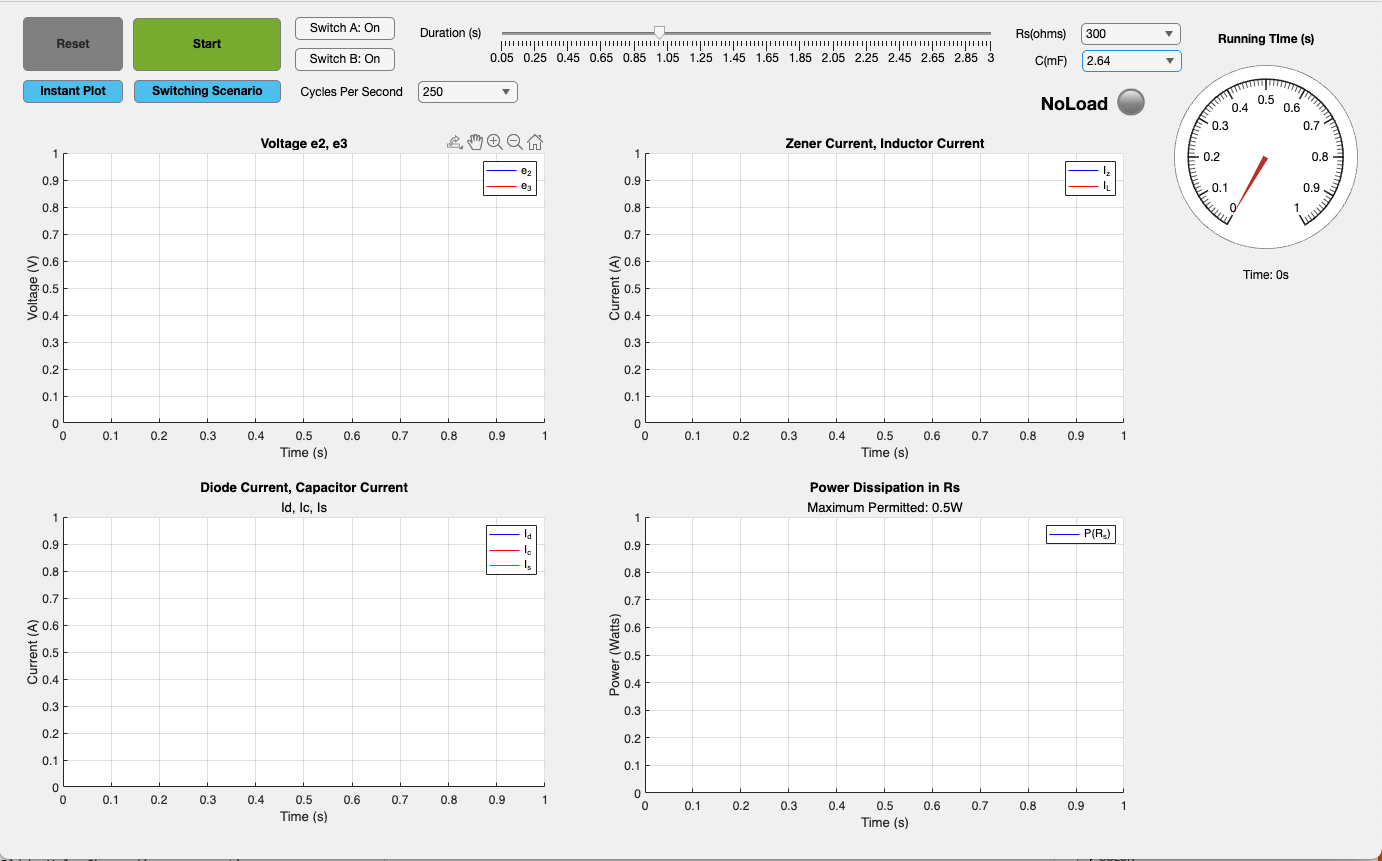
\includegraphics[width=15cm]{graphics/visualisation/inactive_ui}
     \caption{User interface of the visualisation while it is inactive}
\end{figure}
The operation mode of the simulation is determined by the switching of the primary and secondary switches in the multi-mode load, as depicted in Figure \ref{fig:multimode_load}. The user can toggle the switch buttons to change the switching operation dynamically, even while the simulation is running. This enables the user to explore different scenarios and observe the corresponding effects on the circuit's behavior.

\leavevmode\newline
Furthermore, the application supports the adjustment of several parameters. The user can modify the capacitance ($C$) and resistance ($R_s$) values within their nominal, maximum, and minimum ranges, as specified in Table \ref{tab:component_values}. Additionally, the sampling rate ($c$), which determines the time step ($h$) used in the simulation's numerical method (RK4), can be adjusted. Lastly, the user can specify the duration of the simulation, allowing them to observe the circuit's behavior over a desired period.

\leavevmode\newline
To provide real-time feedback to the user, a status indicator is employed to indicate the current mode of operation based on the switch toggles. Additionally, a time gauge is included to keep track of the running simulation time, allowing the user to monitor the progress of the simulation. Control buttons are provided to start, pause, resume, and reset the simulation. These buttons offer convenient control over the simulation's execution and allow the user to pause and resume at any point or start a fresh simulation whenever desired.

\subsection{Implementation}
This MATLAB visualisation application uses AppDesigner to build an interactive user interface for exploring power supply characteristics in different operating modes. It uses a \texttt{ComponentContainer} class which provides a high-level abstraction for the graphical interface, encapsulating the visual components as properties and methods of the class.
\\

Three key functions have been included as code extracts to help illustrate the inner workings and implementation details of the visualisation application. These code snippets highlight specific functions that play crucial roles in enabling the interactive features and simulation capabilities of the application.

\subsubsection{postSetupFcn}
This function, called immediately after the initialization of the application, performs essential setup tasks to configure the initial state of the simulation and prepare the necessary elements for plotting. It establishes the initial conditions, defines the time range, and creates animated lines for each plot.

\begin{lstlisting}[caption=MATLAB code for the function called imeddiately after the UI is initialised]
function postSetupFcn(comp)
% Set initial state
comp.Running = false; 
comp.Paused = false;
comp.t = 0:comp.TimeStep:comp.Duration;
comp.k = 1;
comp.v = @(t) 230 * sqrt(2) * sin(100*pi*t);
comp.ic = [0,0,0];

% Create animated lines for each plot
comp.l_e2 = animatedline(comp.VoltagePlot,Color='b');
comp.l_e3 = animatedline(comp.VoltagePlot,Color='r');
comp.l_iZ = animatedline(comp.VoltagePlot,Color='m');
comp.l_iD = animatedline(comp.DiodeCurrentPlot,Color='b');
comp.l_iC = animatedline(comp.DiodeCurrentPlot,Color='r');
comp.l_iS = animatedline(comp.DiodeCurrentPlot,Color='m');
comp.l_pRs = animatedline(comp.PowerPlot,Color='b');
comp.l_Iz = animatedline(comp.ZenerCurrentPlot,Color='b');
comp.l_Il = animatedline(comp.ZenerCurrentPlot,Color='r');

% Update legends
legend(comp.VoltagePlot, 'e_2', 'e_3');
legend(comp.PowerPlot, 'P(R_s)');
legend(comp.ZenerCurrentPlot, 'I_z', 'I_L');
legend(comp.DiodeCurrentPlot, 'I_d', 'I_c', 'I_s');
end
\end{lstlisting}

\subsubsection{update}
The update function is invoked in response to changes in the circuit's mode, such as switching modes, pausing, resuming, or stopping the circuit. Its primary purpose is to promptly update the user interface (UI) to accurately reflect the current state of the circuit.
\begin{lstlisting}[caption=MATLAB code used to update the UI after a property is changed]
function update(comp)
if ~comp.SwitchingOperation
  if comp.SwitchAOn && comp.SwitchBOn
    comp.Mode = CircuitMode.FullLoad;
  elseif comp.SwitchAOn && ~comp.SwitchBOn
    comp.Mode = CircuitMode.ResistiveLoad;
  elseif comp.SwitchBOn && ~comp.SwitchAOn
    comp.Mode = CircuitMode.InductiveLoad;
  else
    comp.Mode = CircuitMode.NoLoad;
  end
end

comp.NoLoadLampLabel.Text = char(comp.Mode);

if comp.Running
  if comp.Paused
    comp.ModeLamp.Color = [0.502 0.502 0.502];
    comp.StartButton.Text = 'Resume';
    comp.StartButton.BackgroundColor = [0.9294 0.6941 0.1255];
  else
    comp.ModeLamp.Color = 'g';
    comp.StartButton.Text = 'Pause';
    comp.StartButton.BackgroundColor = 'y';
  end
else
  comp.StartButton.Text = 'Start';
  comp.StartButton.BackgroundColor = [0.4667 0.6745 0.1882];
  comp.ModeLamp.Color = [0.502 0.502 0.502];
end
end
\end{lstlisting}

\subsubsection{updatePlot}
This function is utilized in an iterative manner to plot the system parameters from the time index $k$ up to $t_{end}$, which represents the duration of the simulation. The time index $k$, is updated after each iteration, and defined within the interval $$1 \leq t \leq t_{end}$$ When the circuit is paused and subsequently resumed, the current state of the time index is preserved, allowing the circuit to continue the simulation from the exact point where it was paused. This state is stored as a public property within the class.
\begin{lstlisting}[caption=Helper function thats used to simulate the circuit after a given time index $k$]
function finished = updatePlot(comp)
for n=comp.k:length(comp.t)-1
% Stop simulation if no longer running or paused
if ~comp.Running || comp.Paused
break
end

% Get current time from time index, update gague
tn = comp.t(n);
comp.RunningTimesGaugeLabel.Text = ['n: ', num2str(n)];
comp.RunningTimesGauge.Value = tn;
comp.k = n;

% Calcualte t+h and t+h/2 for RK4
tn_1 = tn + comp.TimeStep;
tn_2 = tn + comp.TimeStep / 2;

% Input voltage is a vector
vin = comp.v([tn, tn_1, tn_2]);

% Perform iteration
y = powerSupply(comp.Mode,vin,comp.TimeStep,comp.ic,comp.C,comp.Rs);

% Update initial conditions
comp.ic(1) = y.e2;
comp.ic(2) = y.e3;
comp.ic(3) = y.iL;

% Plot new values on graph
addpoints(comp.l_e2, tn, y.e2);
addpoints(comp.l_e3, tn, y.e3);
addpoints(comp.l_Il, tn, y.iL);
addpoints(comp.l_Iz, tn, y.Iz);
addpoints(comp.l_iD, tn, y.Id);
addpoints(comp.l_iS, tn, y.Is);
addpoints(comp.l_iC, tn, y.Ic);
addpoints(comp.l_pRs, tn, comp.Rs*y.Is.^2)

% Update plot
drawnow limitrate
end
drawnow
finished = comp.k == length(comp.t)-1;
end
\end{lstlisting}

\subsubsection{Auxillary Functions}
Auxiliary functions are used to handle callbacks from user interactions. These include:

\begin{itemize}
    \item \texttt{pause(comp)}: Stops the simulation by setting \texttt{comp.Paused=true}
    \item \texttt{resume(comp)}: Resumes the simulation by setting \texttt{comp.Paused=false}
    \item \texttt{resetSys(comp)}: Resets the simulation by setting all parameters to their initial values (as done in \texttt{postSetupFcn(comp)}) and clearing the existing animated lines.
    \item \texttt{start(comp)}: Starts the simulation and calls \texttt{updatePlot(comp)}. If \texttt{updatePlot()} returns \texttt{true}, \texttt{comp.Running} is set to false to stop the simulation.
\end{itemize}

When control buttons are clicked, these auxiliary functions are called to manage the simulation. Additional functions are defined to handle user inputs, but have been excluded from this report for brevity. 


\pagebreak
\subsection{Usage Guide}
\subsubsection{Buttons}
\begin{figure}[H]
     \centering
     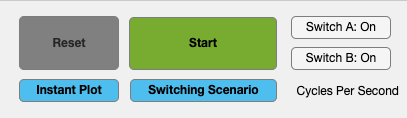
\includegraphics[width=10cm]{graphics/visualisation/ui_buttons}
     \caption{Buttons used in the visualisation interface}
\end{figure}

\paragraph{Switch Buttons}
\begin{itemize}
	\item The "Switch A" and "Switch B" buttons are used to turn on/off the primary and secondary switches in the multi-mode load respectively
	\item Pressing the button once will activate the switch.
	\item Once activated, pressing again will deactivate the switch.
	\item The combination of the switch states is used to determine the mode of operation.
\end{itemize}

\paragraph{Reset} The reset button is used to reset the simulation state. When it is pressed, the user is presented a dialog that the simulation has been reset. 
\begin{figure}[H]
     \centering
     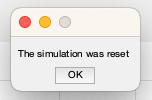
\includegraphics[width=5cm]{graphics/visualisation/dialog_reset}
     \caption{Dialog showing the user that the simulation has been reset}
\end{figure}
Resetting the simulation involves,
\begin{itemize}
	\item Clearing the graphs
	\item Resetting the RK4 initial values
	\item Resetting the time index
	\item Resetting the UI state
\end{itemize}

\paragraph{Start} The start button is used to start the simulation. When it is pressed, the program will begin to solve and plot the differential equations of the system, using RK4 over the specified duration and time step.
When the simulation is active,
\begin{itemize}
	\item The start button changes appearance to a pause button which can be used to stop, and later, resume the simulation
\begin{figure}[H]
     \centering
     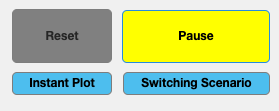
\includegraphics[width=10cm]{graphics/visualisation/pause_button}
     \caption{Dialog showing the user that the simulation has been reset}
\end{figure}
	\item The indicator is updated with a green light to show the simulation is running. The current mode of operation (determined by the switch buttons) is shown in the indicator.
\begin{figure}[H]
     \centering
     \begin{subfigure}[b]{0.45\textwidth}
         \centering
    	 
\includegraphics[width=2.5cm]{graphics/visualisation/ui_indicator_load}
     	\caption{Status indicator of the simulation while it is inactive under no load conditions}
     \end{subfigure}
     \hfill
     \begin{subfigure}[b]{0.45\textwidth}
         \centering
    	 
\includegraphics[width=3.5cm]{graphics/visualisation/ui_indicator_load_active}
     	\caption{Status indicator of the simulation while it is active under an inductive load}
     \end{subfigure}
     \hfill
\end{figure}
\end{itemize}

\paragraph{Instant Plot} Push button which instantly displays the plot at the final time chosen by the user. This plot will remain displayed until the user presses the reset button. 
\begin{figure}[H]
     \centering
     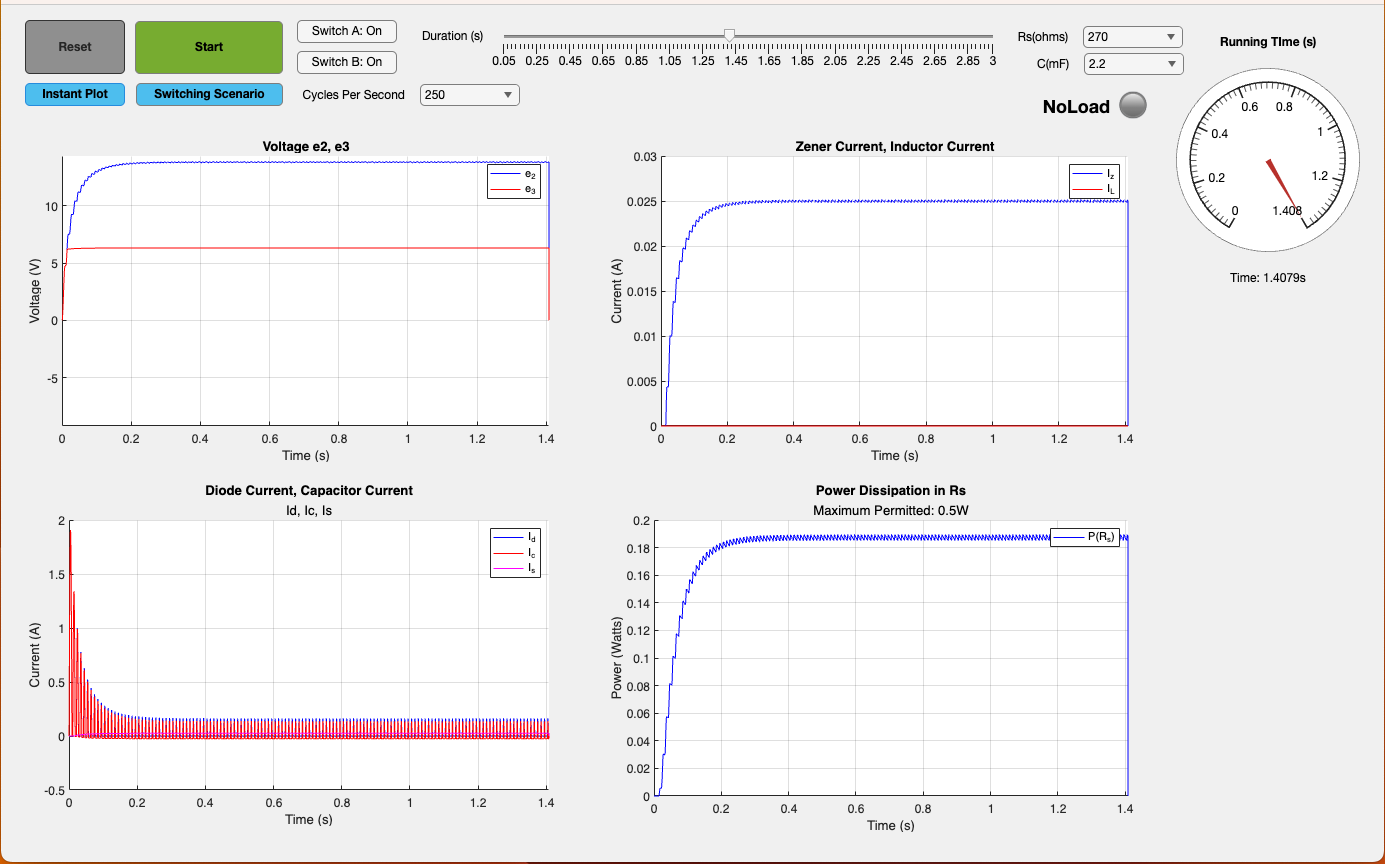
\includegraphics[width=\textwidth]{graphics/visualisation/no_load_instant_plot}
     \caption{The visualisation after pressing the Instant Plot button with no load conditions}
\end{figure}

\paragraph{Switching Scenario} Push button which when activated, triggers the switching scenario detailed in section \ref{section:switchingOperation}

\begin{figure}[H]
   \centering
   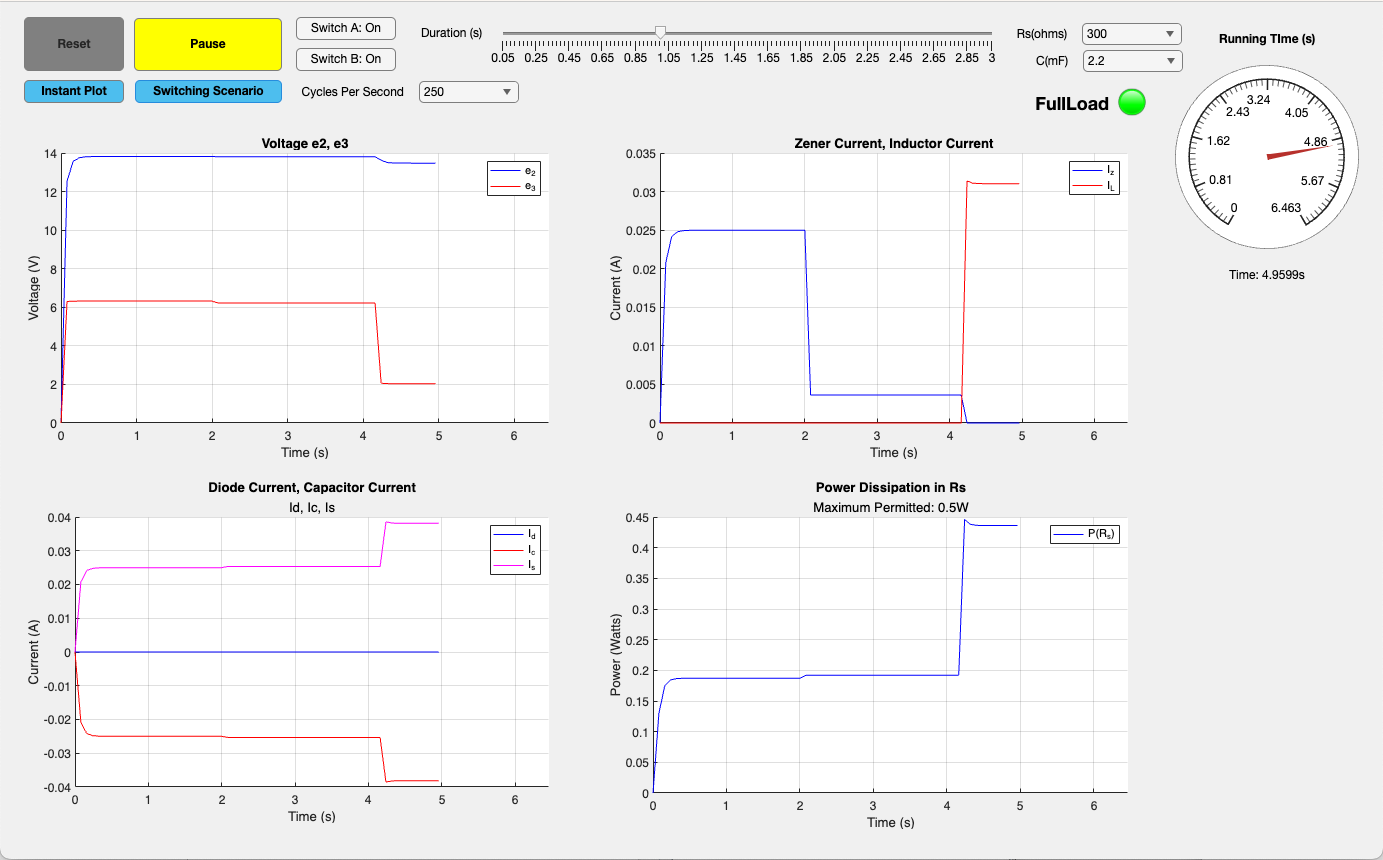
\includegraphics[width=0.95\textwidth]{graphics/visualisation/switching_3}
   \caption{The visualisation a few seconds after pressing the Switching Scenario button}
\end{figure}

\subsubsection{Dropdowns}
\begin{figure}[H]
     \centering
     \begin{subfigure}[b]{0.3\textwidth}
         \centering
    	 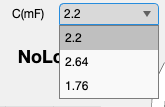
\includegraphics[width=\textwidth]{graphics/visualisation/ui_dropdowns_C}
     	\caption{Drop-down used to control the capacitance $C$ value}
     \end{subfigure}
     \hfill
     \begin{subfigure}[b]{0.3\textwidth}
         \centering
    	 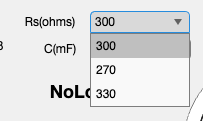
\includegraphics[width=\textwidth]{graphics/visualisation/ui_dropdowns_Rs}
     	\caption{Drop-down used to control the resistance $R_s$ value}
     \end{subfigure}
     \hfill
     \begin{subfigure}[b]{0.3\textwidth}
         \centering
    	 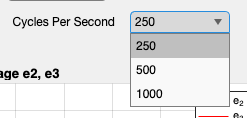
\includegraphics[width=\textwidth]{graphics/visualisation/ui_dropdowns_cycles}
     	\caption{Dropdown used to control the sampling rate $c$. Time step $h$ is determined using $\frac{T}{c}$}
     \end{subfigure}
     \hfill
\end{figure}
These values cannot be modified during the simulation. Doing so will result in the simulation being reset and the user must run the simulation again. A prompt will be shown if a change is detected while the simulation is active.
\begin{figure}[H]
     \centering
     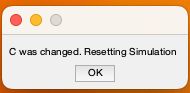
\includegraphics[width=5cm]{graphics/visualisation/dialog_cchange}
     \caption{Dialog showing the user that a change in $C$ was detected}
\end{figure}

\pagebreak
\subsubsection{Duration Slider} A slider which allows the user to change the duration of the simulation 

\begin{figure}[H]
    \centering
   	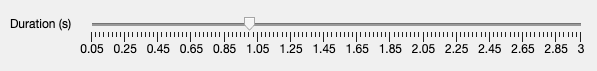
\includegraphics[width=\textwidth]{graphics/visualisation/ui_input_duration}
	\caption{Slider used to control the duration of the simulation}
\end{figure}

\subsubsection{Time Gauge} Working in tandem with the simulation, the time gauge monitors the elapsed time as the simulation advances. This enables the user to maintain a record of the time at specific plot points.

\begin{figure}[H]
    \centering
   	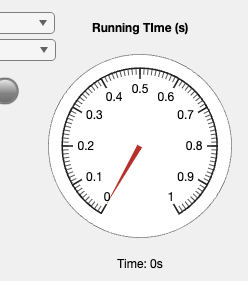
\includegraphics[width=5cm]{graphics/visualisation/ui_indicator_gage}
	\caption{Time gauge used to track the time progression of the simulation}
\end{figure}

\pagebreak
\subsection{Switching Operation} \label{section:switchingOperation}
The Switching Operation push button, integrated into the visualisation interface, serves the purpose of initiating a specific operation that fulfills the following condition
\begin{shquote}
The power supply is switched on at time $t=0$ at which the time the smoothing capacitor voltage and inductor current are zero, neither attached loading device is active at this time; after 2 sec the resistive load is switched on; after a further 2.2 sec the inductive load is switched in (i.e. connected) and it remains connected for the next 1.263 sec; subsequently the inductive device is switched out (i.e. disconnected) and remains disconnected
\end{shquote}

The visualisation was set up to support dynamic switching even while the simulation is running. When the user presses the Switch A and Switch B push buttons, the \texttt{comp.Mode} property is updated accordingly. This updated mode is then applied in the next iteration within the \texttt{updatePlot(comp)} function. Thus, the inductive and resistive loads can be connected and disconnected during the simulation, allowing for real-time changes. Implementing this scenario in the simulation was straightforward. It involved modifying the \texttt{comp.Mode} based on the current time value from the time index $k$.
\begin{table}[H]
    \centering
    \begin{tabular}{|c|c|}\hline
        Time (s) & \texttt{comp.Mode} \\\hline
        $t=0$ & NoLoad \\
        $2 < t < 4.2$ & ResistiveLoad \\
        $4.2 < t < 5.463$ & FullLoad \\
        $t > 5.463$ & ResistiveLoad \\\hline
    \end{tabular}
    \caption{How the \texttt{comp.Mode} value changes with respect to time for this switching operation}
    \label{tab:my_label}
\end{table}
\begin{lstlisting}[caption=Extract of code used to perform switching operation]
% Setup switching scenario
comp.SwitchingOperation = true;
            
% Power supply is switched off at t=0 neither attached loading
% device is active, Ic, IL=0
comp.ic = [0, 0, 0];
comp.Mode = CircuitMode.NoLoad;

% Use a larger time step to speed up
comp.TimeStep = 8e-5;

% Set time interval
t1 = 2; % tn + t1=time when mode=ResistiveLoad
t2 = 2.2; % tn + t2= time when mode=Full load
t3 = 1.263; % time in full load
tend = t1 + t2 + t3 + 1; % total time (add 1s for steady state at end)

% Time breaks
resistiveLoadTime = t1;
fullLoadTime = t1+t2;
revertTime = fullLoadTime+t3;

for n=comp.k:length(comp.t)-1
tn = comp.t(n)

% Check for current mode of operation based on time
if tn >= revertTime
  comp.mode = CircuitMode.ResistiveLoad;
elseif tn >= fullLoadTime
  comp.mode = CircuitMode.FullLoad;
elseif tn >= resistiveLoadTime
  comp.mode = CircuitMode.ResistiveLoad;
else
  comp.mode = CircuitMode.NoLoad;
end
	
% Update vin with time intervals
tn_1 = tn + comp.TimeStep;
tn_2 = tn + comp.TimeStep / 2;
vin = comp.v([tn, tn_1, tn_2]); 

% Perform RK4 simualtion
y = powerSupply(comp.mode,vin,h,comp.ic,comp.C,comp.Rs);  % Perform iteration
   
% Update initial conditions
comp.ic(1) = y.e2;
comp.ic(2) = y.e3;
comp.ic(3) = y.iL;
                
% Plot y-values ... 
end
\end{lstlisting}
\begin{figure}[H]
    \centering
   	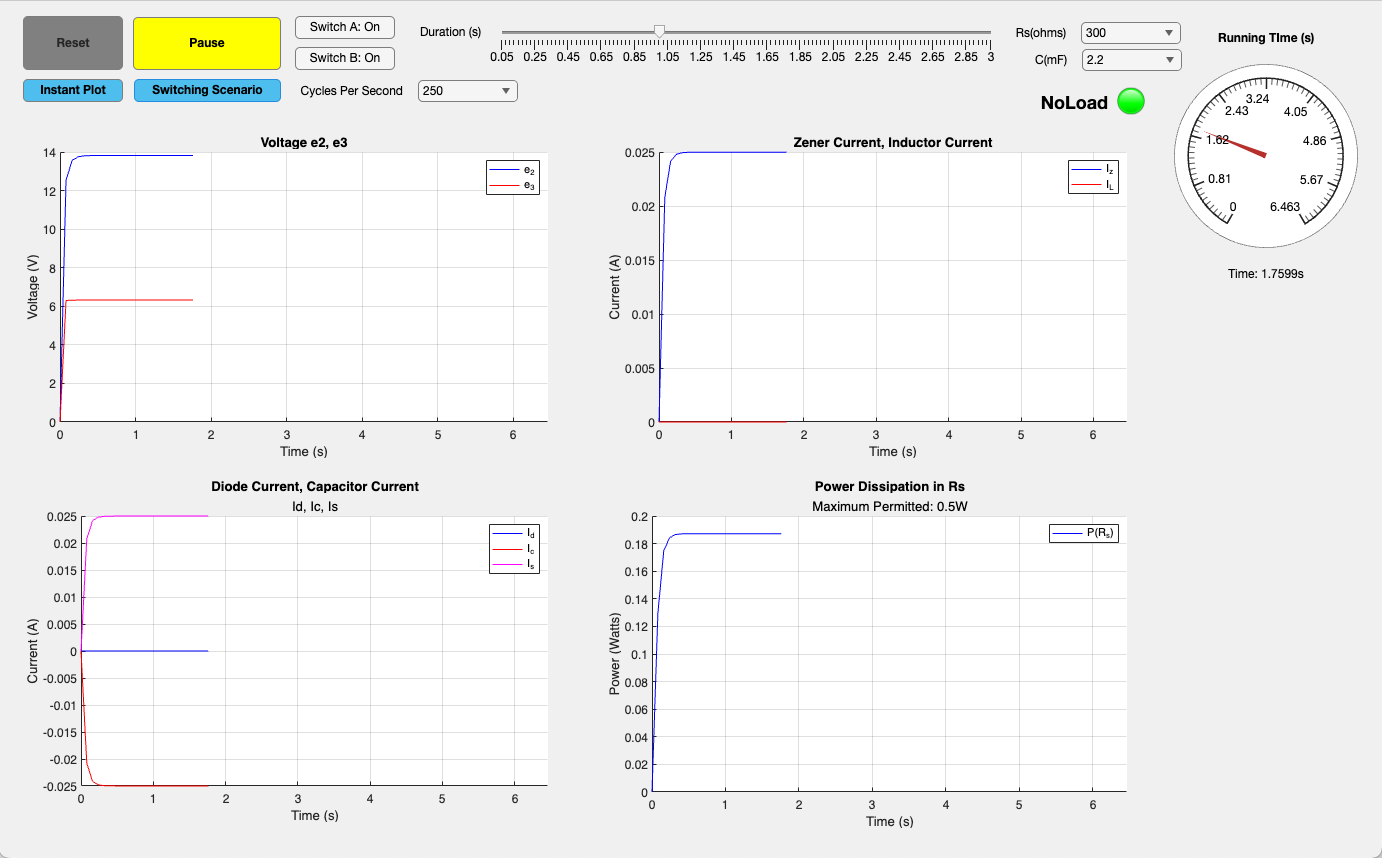
\includegraphics[width=\textwidth]{graphics/visualisation/switching_1}
	\caption{Visualisation at the beginning of the switching operation}
\end{figure}
\begin{figure}[H]
    \centering
   	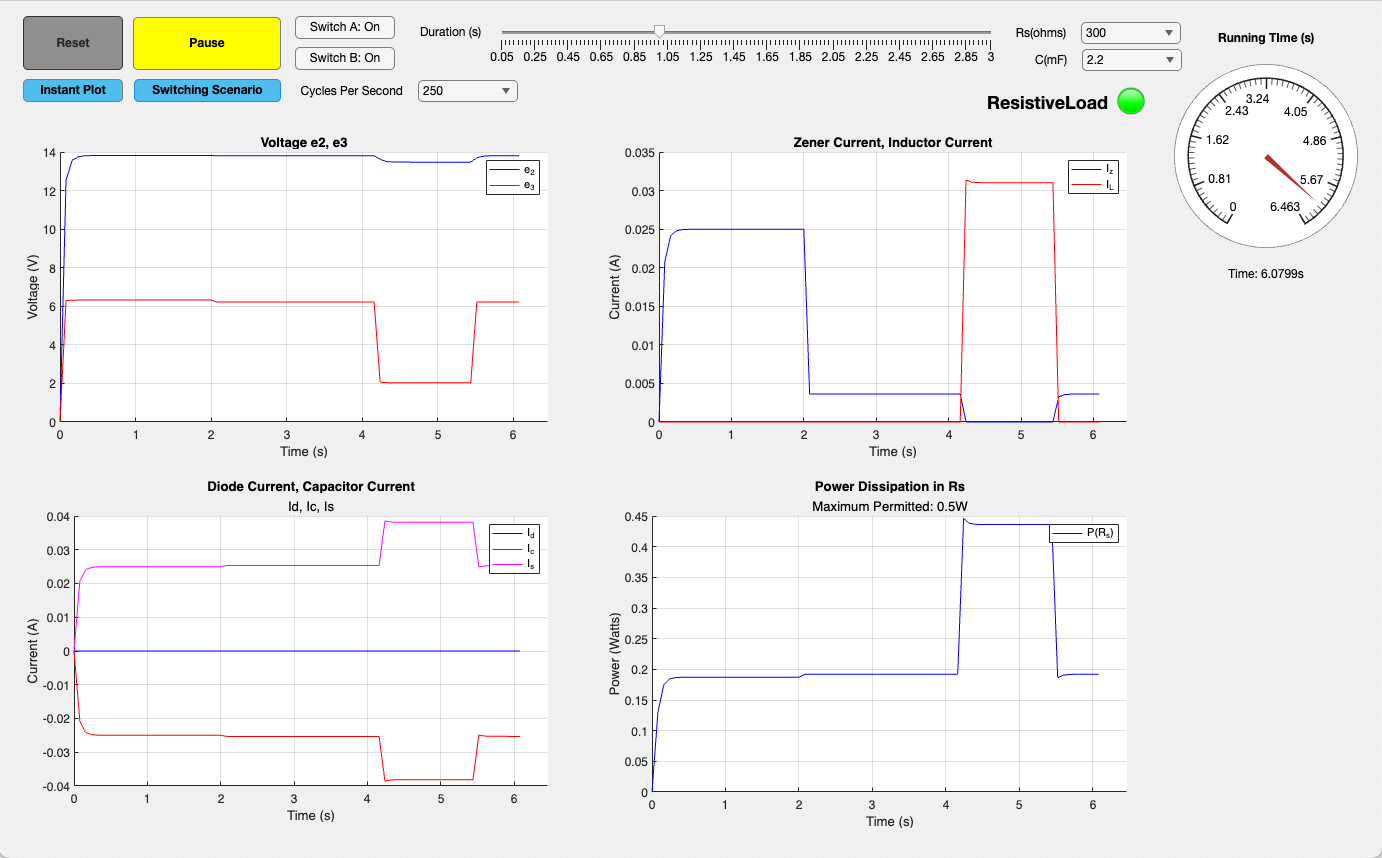
\includegraphics[width=\textwidth]{graphics/visualisation/switching_4}
	\caption{Visualisation towards the end of the switching operation}
\end{figure}
In general, the results of the switching operation align with predictions. After each incident, the circuit enters a transitory phase before stabilising into a consistent state following several cycles. The charge and discharge trajectories of the capacitor align with anticipated outcomes. The inductor's current becomes noticeable only when the inductive load is engaged, and it diminishes slightly upon reaching the stable state.




% S; Appendix
\section*{Appendix}
Add extra notes

% S; Biblography
\bibliography{frontmatter/references}

\end{document}













